% Header
%%%%%%%%%%%%%%%%%%%%%%%%%%%%%%%%%%%%%%%%%%%%%%%%%%%%%%%%%%%%%%%%%%%%%%%%%%%%%%%%
%2345678901234567890123456789012345678901234567890123456789012345678901234567890
%        1         2         3         4         5         6         7         8

\documentclass[letterpaper, 10 pt, conference]{ieeeconf}  % Comment this line out
                                                          % if you need a4paper
%\documentclass[a4paper, 10pt, conference]{ieeeconf}      % Use this line for a4
                                                          % paper

\IEEEoverridecommandlockouts                              % This command is only
                                                          % needed if you want to
                                                          % use the \thanks command
\overrideIEEEmargins
% See the \addtolength command later in the file to balance the column lengths
% on the last page of the document


% The following packages can be found on http:\\www.ctan.org
%\usepackage{graphics} % for pdf, bitmapped graphics files
%\usepackage{epsfig} % for postscript graphics files
%\usepackage{mathptmx} % assumes new font selection scheme installed
%\usepackage{times} % assumes new font selection scheme installed
%\usepackage{amsmath} % assumes amsmath package installed
%\usepackage{amssymb}  % assumes amsmath package installed

\usepackage{advdate,color,soul,amsmath,amssymb,eucal,amscd,graphicx,mathtools}
\let\proof\relax
\let\endproof\relax
\usepackage{amsthm}
\graphicspath{ {images/} }
%\usepackage[utf8]{inputenc}
\let\labelindent\relax
\usepackage{enumitem}

% Theorem styles
\newtheorem{defn}{Definition}

% convenient markup
%d\typesetChapterTitle[1]{#1}
\newcommand{\edit}[1][!!!!!]{\textcolor{red}{\hl{#1}}}
% convenient absolute value
\DeclarePairedDelimiter\abs{\lvert}{\rvert}
\makeatletter
\let\oldabs\abs
\def\abs{\@ifstar{\oldabs}{\oldabs*}} % star prevents auto resize
\makeatother
% convenient space shorthands
\newcommand{\Rone}{\mathbb{R}}
\newcommand{\Rtwo}{\mathbb{R}^{2}}
\newcommand{\Rthree}{\mathbb{R}^{3}}
\newcommand{\Natnums}{\mathbb{N}}
\newcommand{\Integers}{\mathbb{Z}}
% big O notation
\newcommand{\Obig}{\mathcal{O}}
% shortcuts for math notation
\newcommand*{\defeq}{\mathrel{\vcenter{\baselineskip0.5ex \lineskiplimit0pt
			\hbox{\scriptsize.}\hbox{\scriptsize.}}}% personal := format
	=}
\newcommand*{\eqdef}{= % personal =: formatting
	\mathrel{\vcenter{\baselineskip0.5ex \lineskiplimit0pt
			\hbox{\scriptsize.}\hbox{\scriptsize.}}}
}
\newcommand{\bigslant}[2]{{\raisebox{.2em}{$#1$}\left/\raisebox{-.2em}{$#2$}\right.}} % quotient spaces
% complexity theory shortcuts
\newcommand{\Time}{\text{\textbf{TIME}}}
\newcommand{\Space}{\text{\textbf{SPACE}}}
\newcommand{\pspace}{\text{\textbf{PSPACE}}}
\newcommand{\np}{\text{\textbf{NP}}}
\newcommand{\p}{\text{\textbf{P}}}
\newcommand{\exptime}{\text{\textbf{EXPTIME}}}
\newcommand{\expspace}{\text{\textbf{EXPSPACE}}}
% convenient superscripts
\newcommand{\Th}{^{\text{th}}}
\newcommand{\St}{^{\text{st}}}
\newcommand{\Rd}{^{\text{rd}}}
% command for Hausdorff definition
\newcommand{\Hausdorff}[2]{\max\left\{\adjustlimits\sup_{\lowercase{#1}\in #1}\inf_{\lowercase{#2}\in #2}d(a,b)\ ,\ \adjustlimits\sup_{\lowercase{#2}\in #2}\inf_{\lowercase{#1}\in #1}d(a,b)\right\}}
% convenient supinf d() in R
\newcommand{\supinfabs}[2]{\adjustlimits \sup_{\lowercase{#1}\in #1}\inf_{\lowercase{#2}\in #2}\abs{\lowercase{#1}-\lowercase{#2}}}
% convenient margin changing
\def\changemargin#1#2{\list{}{\rightmargin#2\leftmargin#1}\item[]}
\let\endchangemargin=\endlist
% bullet lists without gaps
\newenvironment{myitemize}
{ \begin{itemize}
    \setlength{\itemsep}{0pt}
    \setlength{\parskip}{0pt}
    \setlength{\parsep}{0pt}     }
{ \end{itemize}                  } 

% command for better lists
\newcommand*{\tabulardef}[3]{\begin{tabular}[t]{@{}lp{\dimexpr\linewidth-#1}@{}}
    #2&#3
  \end{tabular}}
\newlength{\standardparindent}
\setlength{\standardparindent}{\parindent}
\newenvironment{minipdef}[2]{\makebox[#1]{#2\ \hfill}%
  \begin{minipage}[t]{\dimexpr\linewidth-#1}%
  \setlength{\parindent}{\standardparindent}\noindent\ignorespaces}%
{\end{minipage}}


\title{\LARGE \bf Encoding Data from libraries.io for Topological Data Analytics}
\author{Brian Friend, Jonathan Anderson, and Kaixiang Wang}


\begin{document}

\maketitle
\thispagestyle{empty}
\pagestyle{empty}


%%%%%%%%%%%%%%%%%%%%%%%%%%%%%%%%%%%%%%%%%%%%%%%%%%%%%%%%%%%%%%%%%%%%%%%%%%%%%%%%
\begin{abstract}

Persistent homology and other forms of topological data analytics are still being developed at a research level, but their use in applications has still been limited. Part of this limitation is from the inability to encode data sets in meaningful ways to apply the techniques. This paper will examine data sets on open-source package managers and compare them using basic TDA tools.

\end{abstract}


%%%%%%%%%%%%%%%%%%%%%%%%%%%%%%%%%%%%%%%%%%%%%%%%%%%%%%%%%%%%%%%%%%%%%%%%%%%%%%%%
\section{INTRODUCTION}

Over the past several decades, new data analysis techniques have been developed using topological theory. By assuming that a data set comes from a distinct topological space, one can describe this data set in terms of a topological invariant. There are several popular invariants, such as a space's homopty, that are not always computationally feasible. For this reason, there have been many efforts to develop polynomial runtime algorithms for calculating different invariants.

A popular algorithm is the calculation of a simplicial complex's homology. The problem with this algorithm alone is that the data used to encode a simplicial complex may be incomplete or erroneous. For this reason, there are techniques used to examine slightly varying encodings of the data to see if the homology {\it persists} throughout. Appropriately named, these calculations are referred to as persistent homology.

Using the same invariant for the topological space of different data sets, one may be able to determine if the topological spaces are distinct. Such a distinction can be used as a way to classify differences in data sets. On the other hand, if two topological spaces share the same value for an invariant, more information would be necessary to determine whether or not they are identical. Since many applications also assume that different data sets come from distinct topological spaces, it is useful to encodings of the data that lead to distinct values for topological invariants. In the case of persistent homology, there have been clear cases where the type of filtrations reveal distinctions in resulting homology. For this study, we will maintain the same type of filtration between data sets, but instead look at how data is initially encoded at the start of the filtration process to see if there is a noticeable affect on persistent homology.

Before going further, some background will be given on the terms used throughout this proposal. In addition to defining the terms, an explanation of their interpretation will be provided.

\section{Background}
\label{sec.background}

\subsection{Simplicial Complexes}
\label{subsec.simcmplx}

Homology is often thought of as the "holes" present in a space. On the real number line, $\Rone$, a hole might be thought of as a missing point; in $\Rtwo$ it might be thought of as a circular gap; and in $\Rthree$ it may be thought of as a three dimensional void in space. Through the theory of singular homology, these notions are generalized to arbitrarily large dimensions and for abstract spaces. Despite being defined on any space, it is only computable on discreet spaces. As we will see, simplicial complexes are discreet spaces which have easily calculated homology.

\begin{defn}
An {\bf $n$-simplex}, $\Delta^n$, is the simplest geometric figure determined by a collection of $n+1$ points in the Euclidean space $\Rone ^n$. That is, it is a complete graph of $n+1$ vertices in $n$ dimensions.
\end{defn}
\begin{defn}
An {\bf $n$-face} of a simplex is a subset of that simplex's vertex set made of $n+1$ vertices.
\end{defn}
\begin{defn}
A {\bf simplicial complex} $\mathcal K$ is a  finite set of simplices satisfying the following conditions:
\begin{myitemize}
\item For each simplex $A\in\mathcal K$, every face of $A$ is also a simplex of $\mathcal K$; and
\item for $A,B\in \mathcal K$, either $A\cap B$ is empty or it is a shared face.
\end{myitemize}
\end{defn}

So a simplicial complex is a space with nice features defined on a finite subset of the power set of a finite set of points. Because empirical data sets are finite, it is natural to use this set as the foundation for a simplicial complex. These points are often referred to as the {\it vertices} of the complex.

%Homology defs
\subsection{Simplicial Homology}
\label{subsec.simhomo}

Before being able to calculate simplicial homology, there must be an orientation on the vertices of a simplex. This can be thought of as an ordering of the vertices such that an equivalence relation is defined for all orderings that differ by an even permutation.

\begin{defn}
A {\bf simplicial $k$-chain} is given by a sum $$\sum\limits_{i=0}^k c_i\sigma_i$$ where each $c_i$ is an integer and $\sigma_i$ is an oriented $k$-simplex.
\end{defn}
\begin{defn}
	The {\bf group of $k$-chains} on a simplicial complex, written $C_k$, is a free abelian group with a basis in one-to-one correspondence with the set of $k$-simplices in the complex.
\end{defn}
\begin{defn}
	The {\bf boundary operator} is a function\\
	$\delta_k:C_k \rightarrow C_{k-1}$ given such that 
\end{defn}

\section{Goals}
\label{sec.goals}

There were several desired outcomes expected from the completion of this study. Primarily, it was started to expose the investigators to software libraries for using persistent homology, and to provide more comfort in using this form of data analytics.

The larger objective (and the one that persisted despite a significant team/focus reshuffling) was to discover any underlying differences to the structure of software package managers. Beyond the obvious mismatches such as name and author, there may be a way to track the philosophy, coding style, and contributions of an open-source package managers. Some software is meant to be self contained while others rely heavily on previously written software. Rather than asking every software author their philosophy and determining how closely their code matches, it is more practical to examine large collections of software written among a complete package manager.

By using topological data analytics on these large data sets, the study will determine if there is an appropriate way to encode data such that the differences in package managers and structural philosophy can be quantified. This will be especially interesting when comparing the results to the natural graph structure created from package dependencies. This information is included in the original data, but it is unknown how to best represent these dimensions so that our tools will be able to pick up on them.

\section{Motivation}
\label{sec.methods}

There are many software libraries that exist for calculating persistent homology such as Perseus, Ripser, JavaPlex, and Dionysus. This project primarily relied on Cytoscape and the R package called {\it TDA: Statistical Tools for Topological Data Analysis}, respectively, for its graph presentation and analytics.

The data itself was pulled from \emph{libraries.io} which monitors millions of open-source project libraries and dozens of package managers while keeping track of dependency, version, and requirement information. We extracted six subsets of this much larger database, namely the CRAN, Elm, Pub, Dub, Hex, and Haxelib package managers. From there we spent a significant amount of our time cleaning out information that was irrelevant to structure (e.g. package author and creation date) and analyzing what important information remained.

It is important that the method for constructing simplicial homologies and the type of filtration act as the control variables for this experiment. First, a convenient filtration will need to be set up for the size of the data sets. Experiments will be carried out on how the data is encoded. Different dimensions of the original data will be included/excluded, and several values may be artificially calculated before being included as dimensions to the data. An example of a possible calculated dimension would be the out-degree from a package's dependency tree. It would be interesting if this value alone was enough to quantify the topological differences between data sets. So the study will test both the types of dimensions and the quantity of dimensions used for calculating persistence barcodes.

Originally, we planned on calculating persistence barcodes from each data set, and then their the bottleneck and/or Wasserstein distances. 
If these distances are sufficient, then it may suggest that the encoding is appropriate for using the tool. 
Should some encodings induce greater pair-wise distances, we may examine the cause and determine which is the most appropriate for our data.
However, due to the exit of our team leader, we refocused our attention on analyzing basic dependency information from graph statistics using R and Cytoscape.

\section{RESULTS \& DISCUSSION}

Graphing the structure of a dependency tree required significant filtering to produce meaningful results:
	redundant information like Dependency Platform and Dependency Kind were removed 
	(with no meaningful change to the end result) to significantly speed up graph creation, 
    and version information (Version ID, Version Requirements, etc.) resulted in multigraphs 
	that significantly obfuscated the relationships we were after.

Our graphs used Dependency Name as Source (with Dependency Project ID as the most important Source attribute)
and Project Name as the Target (with Project ID as the most important Target attribute)

%%%%%%%%%%%%%%%%%%%%%%%%%%%%%%%%%%%%%%%%%%%%%%%%%%%%%%%%%%%%%%%%%%%%%%%%%%%%%%%%

\subsection{Elm, CRAN, Pub}

The graphs produced by analyzing the Elm, CRAN, and Pub data 
	typify the densely clustered package managers monitored by \emph{libraries.io}:
	high Node Count, Centralization, and Coefficient of Clustering;
	and small Path Lengths with more Connected Components.

\begin{center}
\begin{tabular}{||c c c c c c ||} 
\hline
Pub & 7.769 & 2484 & 0.382 & 0.413 & 12  \\ 
\hline
PM & Neigh. & Nodes & Centr. & Clust. & NComp. \\ [0.5ex] 
\hline\hline
CRAN & 9.721 &	10438 & 0.617 & 0.3038 & 14 \\ 
\hline
Elm & 5.329 & 900 & 0.993 & 0.572 & 1 \\ [1ex] 
\hline
\end{tabular}
\end{center}

And at the low end of this highly-clustered group,
	we have Pub, the package manager for the Dart programming language 
    (itself a very young language that first appeared in 2011). 
    Its results -- in particular its Centralization and Clustering hovering around 50\%, 
    and its ratio of Connected Components to the Node Count not passing 1\% -- 
    are fairly typical for the medium-aged package managers,

Going into this project, we expected CRAN to exhibit the highest level of clustering:
	because R is (as far as languages go) ancient
    and benefits from a large and active community of open-source developers: 
    age and community size (as proxied by Node Count) would drive "closeness".

The attached graph and data seemed to match our expectations, 
	but to our surprise we found that the package manager for the Elm programming language 
	produced the most densely clustered dependency graph. 
    Despite its youth (it first appeared in 2012),
    it beat CRAN at Centralization and Coefficient of Clustering, 
    while producing only 1 Connected Component to CRAN's 14.
    In other words, a language's age and the size of the community behind it
    did not seem to be the sole drivers of clustering.

\begin{figure} % Pub
\centering
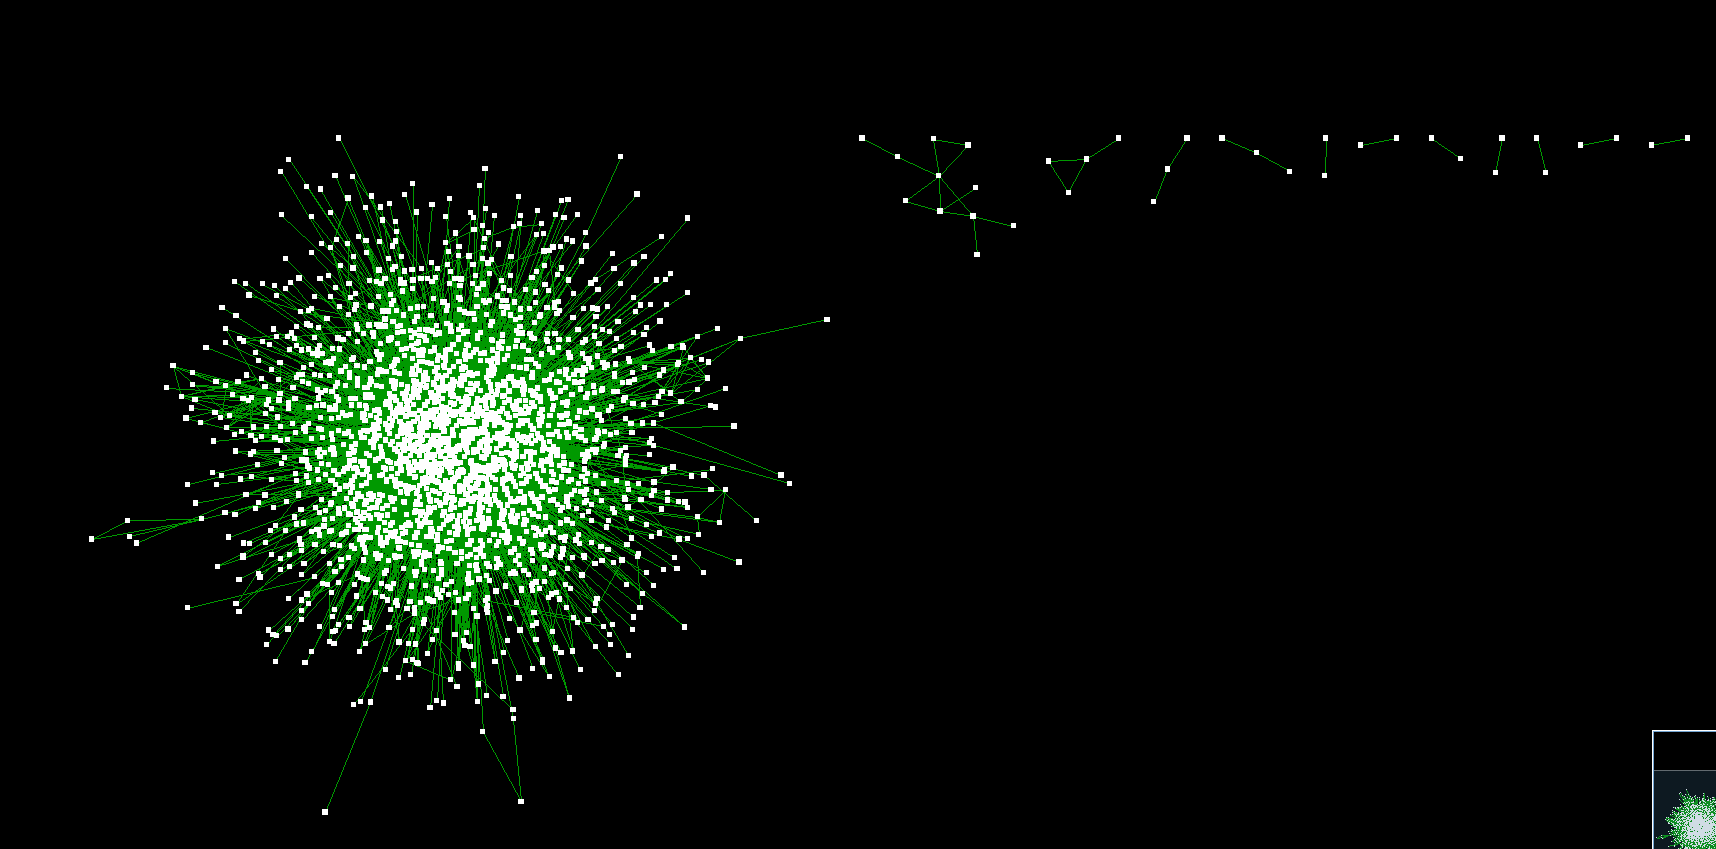
\includegraphics[width=3in]{images/Pub_Graph.png}
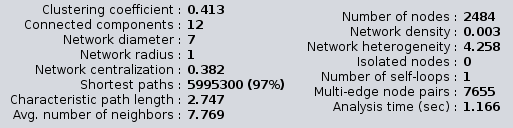
\includegraphics[width=3in]{images/Pub_Params_Screenshot.png}
\caption{\label{Pub_Graph} structure of Pub dependencies}
\end{figure}

\begin{figure} % CRAN
\centering
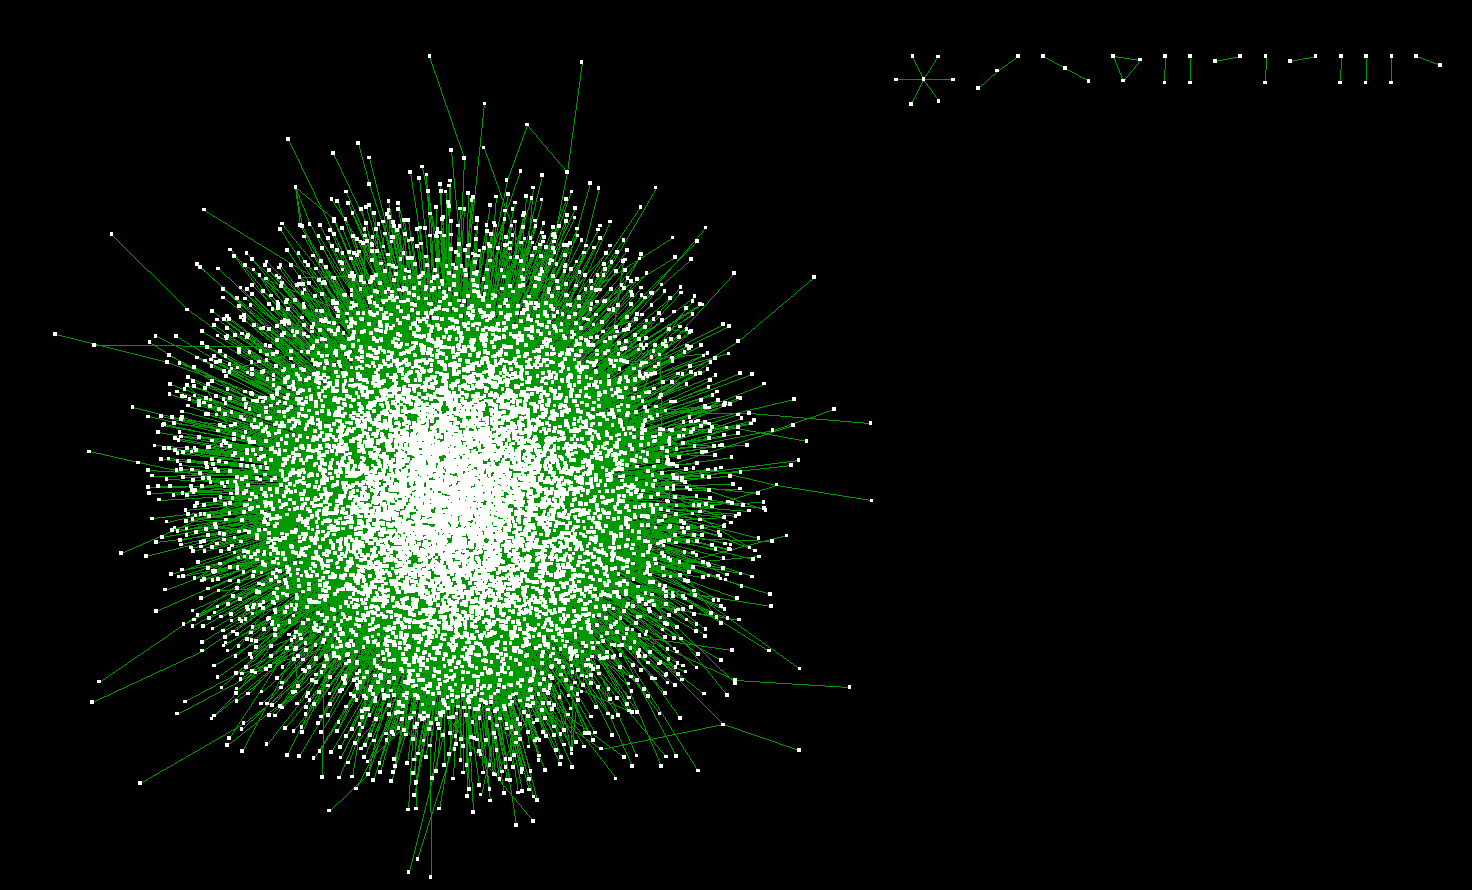
\includegraphics[width=3in]{images/CRAN_Graph.png}
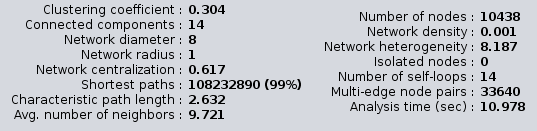
\includegraphics[width=3in]{images/CRAN_Params_Screenshot.png}
\caption{\label{CRAN} structure of CRAN dependencies}
\end{figure}

\begin{figure} % ELM
\centering
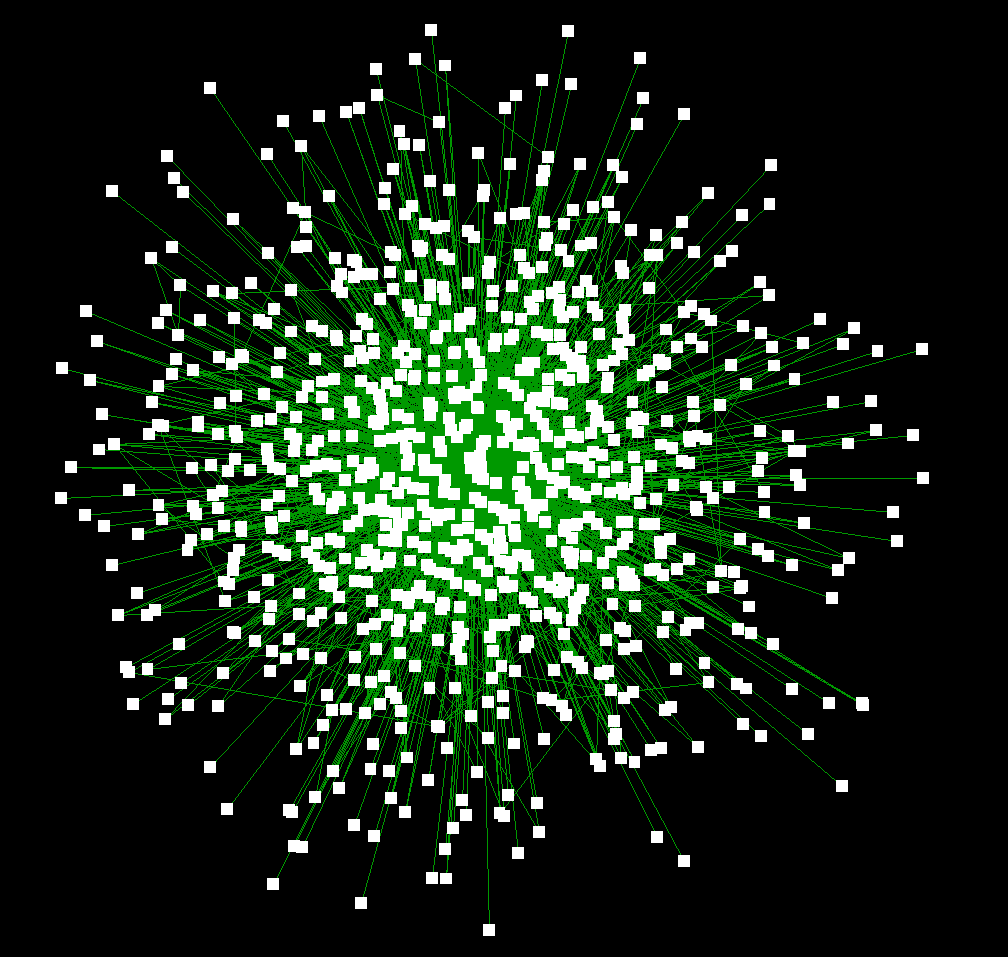
\includegraphics[width=3in]{images/Elm_Graph.png}
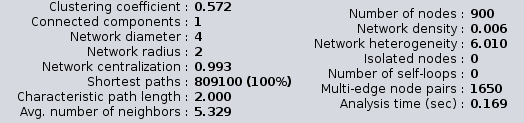
\includegraphics[width=3in]{images/Elm_Params_Screenshot.png}
\caption{\label{Elm_Graph} structure of Elm dependencies}
\end{figure}

%%%%%%%%%%%%%%%%%%%%%%%%%%%%%%%%%%%%%%%%%%%%%%%%%%%%%%%%%%%%%%%%%%%%%%%%%%%%%%%%

\subsection{Hex, Dub, Haxelib}

In contrast to the package managers that produced densely clustered graphs,
the next three package managers' graphs are characterized 
by low values in Node Count, Centralization, Coefficient of Clustering,
and larger values in Path Length and Connected Components. 
These package managers represent open-source communities 
that are less closely connected and with more pockets of isolated development.

\begin{center}
\begin{tabular}{||c c c c c c ||} 
\hline
PM & Neigh. & Nodes & Centr. & Clust. & NComp. \\ [0.5ex] 
\hline\hline
Hex & 4.021 &	2993 &	0.265 &	0.103 & 72 \\ 
\hline
Dub & 2.515 &	684	& 0.126 &	0.103 &	54 \\
\hline
Haxelib & 2.544 & 706 & 0.102 & 0.000	& 52  \\ [1ex] 
\hline
\end{tabular}
\end{center}

Hex is the package manager for the Erlang programming language and garbage-collection runtime system.
	Its age (Erlang first appeared in 1986) might explain the similarities to Pub, CRAN, and Elm:
    for these three PMs, Hex exhibits relatively high Centralization (it "looks" much closer to Pub than Haxelib, for instance), 
    but its sheer number of Components as well as its poor Coefficient of Clustering 
    mean Hex has far more in common with the poorly clustered Package Managers.

Dub is the D programming language's official package manager, 
	and the language's relative youth (it was first released only in 2001)
    shows in the graph's non-centrality and high number of connected components.
	As we discovered previously, however, the youth of a language and its community are not the end of the story. 
    Elm's graph was much denser and had more centrality despite only being introduced in 2012. 

Haxelib is the package manager for the Haxe toolkit, 
	and the data on its package manager produced a graph with the lowest levels of Centralization and Clustering, 
    but (surprisingly) not the largest number of Connected Components or smallest Average Neighbor count.
    That is, Haxelib's structure represents a community that is more spread out than the others,
    with its development groups more isolated than those of Dub or Hex.
    
\begin{figure} % HEX
\centering
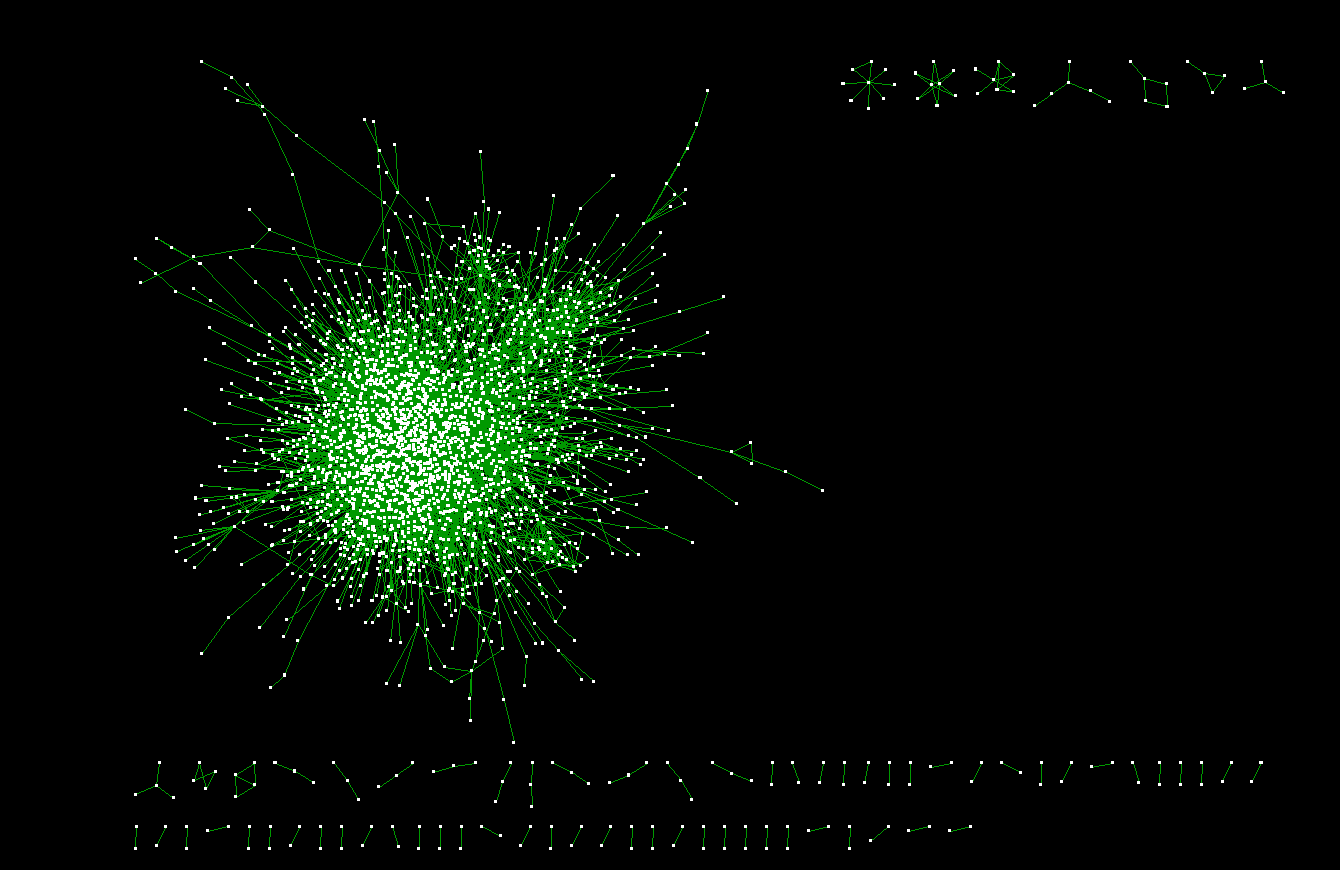
\includegraphics[width=3in]{images/Hex_Graph.png}
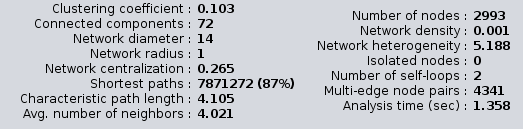
\includegraphics[width=3in]{images/Hex_Params_Screenshot.png}
\caption{\label{Hex_Graph} structure of Hex dependencies}
\end{figure}

\begin{figure} % DUB
\centering
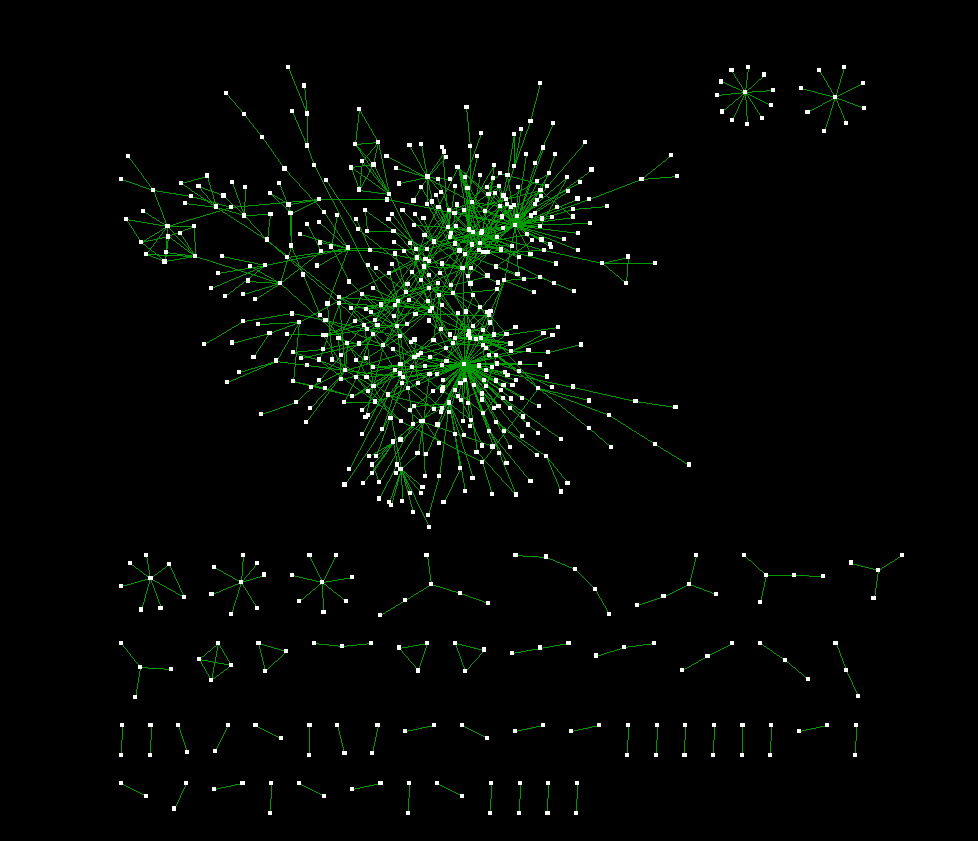
\includegraphics[width=3in]{images/Dub_Graph.png}
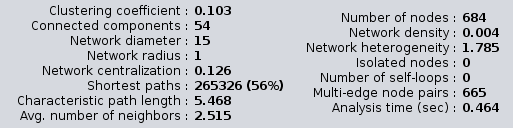
\includegraphics[width=3in]{images/Dub_Params_Screenshot.png}
\caption{\label{Dub_Graph} structure of Dub dependencies}
\end{figure}

\begin{figure} % HAXELIB
\centering
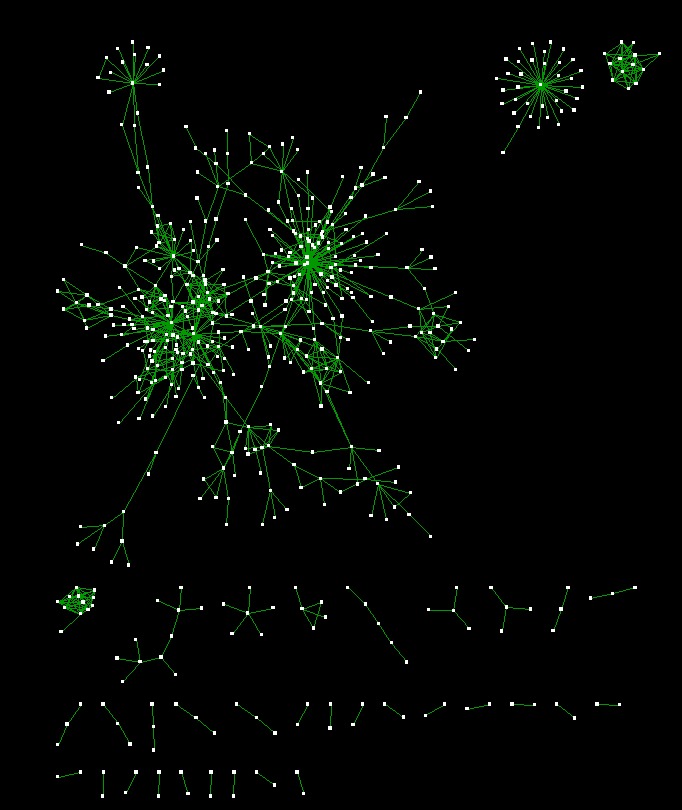
\includegraphics[width=3in]{images/Haxelib_Graph.png}
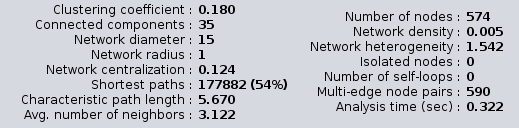
\includegraphics[width=3in]{images/Haxelib_Params_Screenshot.png}
\caption{\label{Haxelib_Graph} structure of Haxe dependencies}
\end{figure}

%%%%%%%%%%%%%%%%%%%%%%%%%%%%%%%%%%%%%%%%%%%%%%%%%%%%%%%%%%%%%%%%%%%%%%%%%%%%%%%%

\end{document}
